\subsubsection{Gaussian Process}
\label{appendix:GP}

Linear models [\cref{appendix:linear_regression}] are fundamentally constrained by their linearity, in which the only degree of freedom comes from the parameters to be optimised. The introduction of kernels in KRR [\cref{appendix:krr}] partially alleviated this problem through the use of kernel functions that implicitly encode non-linear relationships among the features, but a linear relationship between the features and the target variable is still assumed. In this regard, GP regression is the most flexible non-parametric Bayesian regression model, which move from optimisating the probability distribution over the model parameters to a regime of optimising the probability distribution over the space of functions $\{f(\bm{x})\}$ to arrive at the best surrogate model to fit the underlying data [\cref{fig:GP_illustration}].

\begin{figure}[htb]
    \centering
    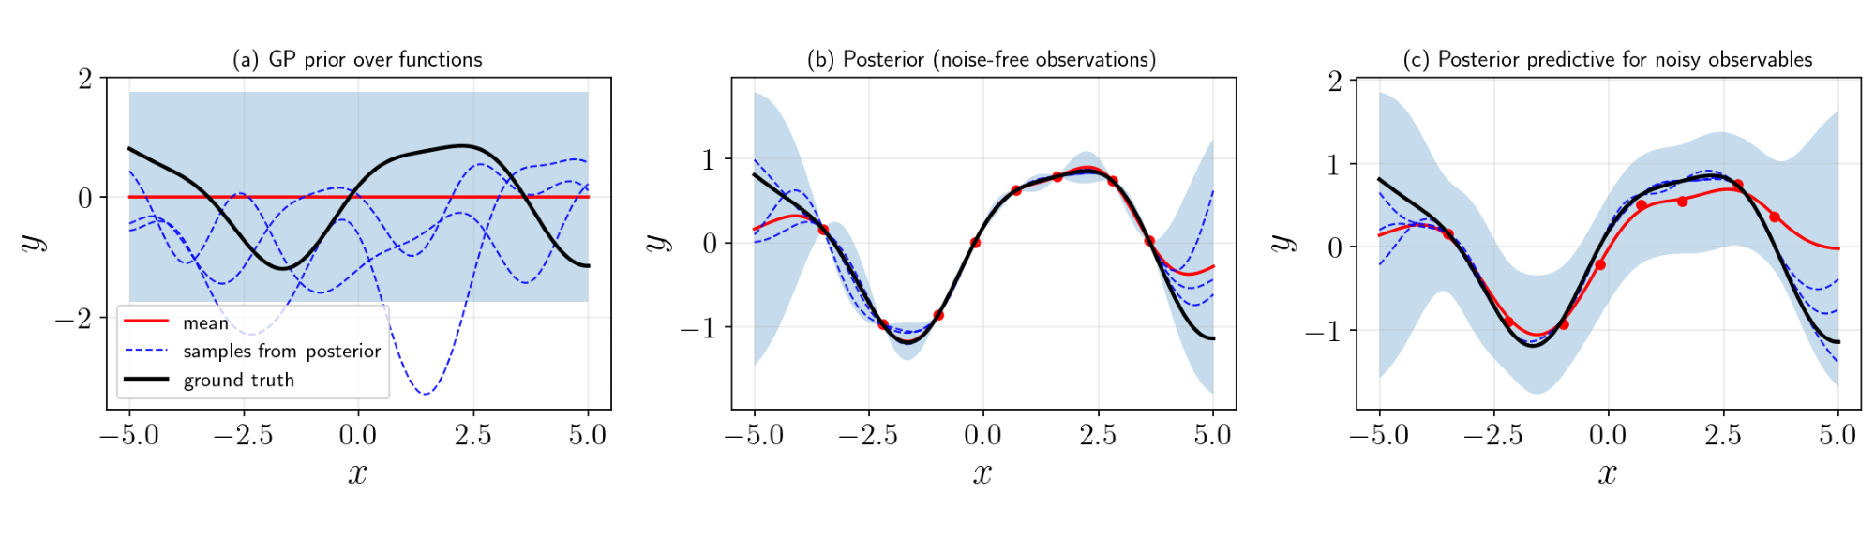
\includegraphics[width=\textwidth]{GP_illustration.pdf}
    \caption{Graphical illustration of the GP regression process to fit a set of data points (red dots) that are drawn from an underlying ground truth function (solid black curve). (a) The prior distribution over functional space that is defined by the mean (red solid curve) and the covariance (shaded area) of the GP, with a few samples drawn from the prior distribution (dashed blue curves). The posterior distribution over the functional space after observing the data points after training the GP model with noise-free (b) and noisy (c) data points. For noise-free data points, the posterior mean of the function passes exactly through the data points with small prediction uncertainties (i.e. small shaded area) around the data points, which is a constraint that is relaxed when fitting the  noisy data points.}
    \label{fig:GP_illustration}
\end{figure}

In this case, the prior distribution in the GP regression is no longer one that is defined over the parameter space [\cref{eq:linear_ridge_param_prior}] but over the function space. To start, for a set of data $\{(\bm{x}_i,y_i)\}_{i=1}^N$, $\bm{x}\in\mathbb{R}^d$ and $y\in\mathbb{R}$, we define the prior distribution over the function space as a Gaussian Process from which plausible functions can be sampled, which is fully specified by a mean function $m(\cdot)$ and a covariance function (or kernel) $k(\cdot,\cdot)$ as follows:
\begin{equation}
    \label{eq:GP_function_prior}
    f(\cdot)\sim\mathcal{GP}\big(m(\cdot),k(\cdot,\cdot) \big).
\end{equation}
Practically, a given function is represented as a finite-dimensional vector $\bm{f}=[f(\bm{x}_1),f(\bm{x}_2)\ldots,f(\bm{x}_N)]^\top\in\mathbb{R}^N$ evaluated at the training data points, which is drawn from a multivariate Gaussian distribution $\bm{f}\sim\mathcal{N}(\bm{m},\bm{K})$, in which: (a) The mean vector $\bm{m}$ has the entries $m_i=m(\bm{x}_i)$, which is some function of the input $\bm{x}_i$ but is often set to zero for simplicity after centering $\{y_i\}_{i=1}^N$ around zero. (b) The kernel matrix $\bm{K}$ has the entries $K_{ij}=k_{\boldsymbol{\varphi}}(\bm{x}_i,\bm{x}_j)$, which is positively defined and encodes some prior belief on how strongly the function values at $\bm{x}_i$ and $\bm{x}_j$ are correlated with each other (i.e. whether we expect $f(\bm{x})$ to be a widly oscillating or a smooth function). The kernel function is often parameterised by a set of hyperparameters $\boldsymbol{\varphi}$, which can be optimised by maximising the marginal likelihood of the data, or may need to be separatedly optimised, depending on the form of the kernel function $k_{\boldsymbol{\varphi}}$.

One of the key advatanges of GP is that it encourages the incorporation of the information of noises in the target variable $y$, that can be concurrently accounted during the model training. In this case, we first rewrite $\{(\bm{x}_i,y_i)\}_{i=1}^N$, $\bm{x}\in\mathbb{R}^d$ as $\{\bm{X},\bm{y}\}$ with $\bm{X}=(\bm{x}_1,\bm{x}_2\ldots,\bm{x}_N)^\top\in\mathbb{R}^{N\times d}$ and $\bm{y}=(y_1,y_2\ldots,y_N)^\top\in\mathbb{R}^N$, from which we can replace $\bm{y}$ by its noised version $\bm{y}^\prime=\bm{y}+\varepsilon\bm{I}$, where we assumed that the noise $\varepsilon$ is a single scalar drawn from a Gaussian distribution $\varepsilon\sim\mathcal{N}(0,\sigma^2)$ with zero mean and variance $\sigma^2$ (a hyperparameter to be optimised). Although there is nothing stopping us from assuming a more complex sample-dependent noise model by having $\boldsymbol{\sigma}^2=\mathrm{diag}\{\sigma^2_1,\sigma^2_2,\cdots,\sigma^2_N\}$.

From here, the primary goal of optimising the GP model is to maximise the probability distributions of the target observables conditioned on the input data and model parameters, \emph{i.e.} $p(\bm{y}^\prime\vert \bm{X},\boldsymbol{\varphi},\sigma^2)$. To align with the viewpoint of optinmising the distribution over the function space, we can use the fact that the conditional distribution $p(\bm{y}^\prime\vert \bm{X},\boldsymbol{\varphi},\sigma^2)$ can be obtained by margionalised over all possible functions whose distribution is conditioned on the data and model parameters, such that:
\begin{equation}
    \label{eq:GP_marginal_likelihood}
    p(\bm{y}^\prime\vert \bm{X},\boldsymbol{\varphi},\sigma^2)=\int p(\bm{y}\vert\bm{f},\sigma^2)p(\bm{f}\vert\bm{X},\boldsymbol{\varphi})\mathrm{d}\bm{f},
\end{equation}
in which $p(\bm{f}\vert\bm{X},\boldsymbol{\varphi})\sim\mathcal{N}(\bm{m},\bm{K}_{\boldsymbol{\varphi},\sigma})$, where $\bm{K}_{\boldsymbol{\varphi},\sigma}=\bm{K}_{\boldsymbol{\varphi}}+\sigma^2\bm{I}$. Without elaborating on the details of the derivation,\cite{williams2006gaussian} the logarithm of the marginal likelihood, which is the objective function to be maximised, can be expressed as:
\begin{equation}    \label{eq:GP_log_marginal_likelihood}
    \mathcal{L}(\boldsymbol{\varphi},\sigma^2)=-\frac{1}{2}\bm{y}^{\prime\top}\bm{K}_{\boldsymbol{\varphi},\sigma}^{-1}\bm{y}^\prime-\frac{1}{2}\log\vert\bm{K}_{\boldsymbol{\varphi},\sigma}\vert-\frac{N}{2}\log 2\pi.
\end{equation}  
The first term in \cref{eq:GP_log_marginal_likelihood} is the data fit term, which encourages the model to fit the data well, while the second term is the complexity penalty term, which penalises models that are too complex (i.e. with a large kernel matrix determinant). The third term is a constant that does not depend on the model parameters and can be ignored during optimisation. 

To optimise $\mathcal{L}(\boldsymbol{\varphi},\sigma^2)$ defined in \cref{eq:GP_log_marginal_likelihood}, one typically first apply the Cholesky decomposition to $\bm{K}_{\boldsymbol{\varphi},\sigma}$ to obtain $\bm{L}\bm{L}^\top=\bm{K}_{\boldsymbol{\varphi},\sigma}$, which allows us to compute the inverse and determinant of $\bm{K}_{\boldsymbol{\varphi},\sigma}$ efficiently. More specficially, the inverse can be computed by first solving the eigenvalue problem of $\bm{L}\bm{v}=\bm{y}^\prime$ from which $\bm{L}^\top\boldsymbol{\alpha}=\bm{v}$ or $\boldsymbol{\alpha}=\bm{K}_{\boldsymbol{\varphi},\sigma}^{-1}\bm{y}^\prime$, and the determinant can be computed as $\vert\bm{K}_{\boldsymbol{\varphi},\sigma}\vert=\vert\bm{L}\vert^2=\prod_{i=1}^N L_{ii}^2$, such that $\log\vert\bm{K}_{\boldsymbol{\varphi},\sigma}\vert=2\sum_{i=1}^N \log L_{ii}$. With these efficient computations, the gradient of $\mathcal{L}(\boldsymbol{\varphi},\sigma^2)$ with respect to the model parameters can be computed as:
\begin{equation}    \label{eq:GP_log_marginal_likelihood_gradient}
    \frac{\partial\mathcal{L}}{\partial\boldsymbol{\varphi}}=\frac{1}{2}\mathrm{tr}\bigg(\big(\boldsymbol{\alpha}\boldsymbol{\alpha}^\top-\bm{K}_{\boldsymbol{\varphi},\sigma}^{-1}\big)\frac{\partial\bm{K}_{\boldsymbol{\varphi},\sigma}}{\partial\boldsymbol{\varphi}}\bigg),\quad\frac{\partial\mathbf{K}_{\boldsymbol{\varphi},\sigma}}{\partial\sigma^2}=\bm{I}.
\end{equation}
An interesting point to note is that, with the optimised kernel, we have $\boldsymbol{\alpha}=\hat{\bm{K}}^{-1}\bm{y}$, which is the same as the solution of KRR [\cref{eq:KRR_optimum_solution}] with $\lambda=0$. This is because, with the optimised kernel, the GP regression can be viewed as a KRR with a kernel that is optimised to fit the data well, which is equivalent to a KRR with a fixed kernel and zero regularisation. However, it is important to note that the optimisation of the kernel in GP regression is not equivalent to the optimisation of the regularisation parameter in KRR, as they are two different aspects of the model.

To make the predictions with the trained GP model, we start from a set of training data $\{(\bm{x}_i,\bm{y}_i)\}_{i=1}^{N}$ and a set of predictive inputs $\{\bm{x}_*\}_{i=1}^M$. From here, we have the mean of the distribution of the predictive function values $m(\bm{X})=\bm{m}\in\mathbb{R}^N$ and $m(\bm{X_*})=\bm{m}_*\in\mathbb{R}^M$. Correspondingly, we have three sets of kernel matrices: $\hat{\bm{K}}\in\mathbb{R}^{N\times N}$, $\hat{\bm{K}}_{*}\in\mathbb{R}^{N\times M}$ and $\hat{\bm{K}}_{**}\in\mathbb{R}^{M\times M}$, which are computed by evaluating the kernel function amongst the training data points, between the training data points and the predictive inputs, and amongst the predictive inputs, respectively. These ingredients leads to the following joint probability distribution of the training and predictive function values:
\begin{equation}    \label{eq:GP_predictive_distribution}
    \begin{bmatrix}\bm{f}\\\bm{f}_*
    \end{bmatrix}\sim\mathcal{N}\bigg(
    \begin{bmatrix}\bm{m}\\\bm{m}_*
    \end{bmatrix},
    \begin{bmatrix}\hat{\bm{K}}&\hat{\bm{K}}_*\\\hat{\bm{K}}_*^\top&\hat{\bm{K}}_{**}
    \end{bmatrix}\bigg).
\end{equation}
By properly centering the data thus making $\bm{m}=\bm{m}^*=0$, this gives us the probability distribution of the predictive function values $\bm{f}_*$ that pass through the predictive inputs $\{\bm{x}_*\}_{i=1}^M$ as follows:
\begin{equation}    \label{eq:GP_predictive_distribution_final}
    p(\bm{f}_*\vert\bm{X},\bm{y},\boldsymbol{\varphi},\sigma^2)\sim\mathcal{N}\Big(\hat{\bm{K}}_*^\top(\hat{\bm{K}}+\sigma^2\bm{I})^{-1}\bm{y},\hat{\bm{K}}_{**}-\hat{\bm{K}}_*^\top(\hat{\bm{K}}+\sigma^2\bm{I})^{-1}\hat{\bm{K}}_*\Big).
\end{equation}
and correspondinly the point prediction at $\bm{x}_*$ and its associated uncertainty can be obtained by the mean and variance of the predictive distribution as:
\begin{equation}    \label{eq:GP_predictive_single_point}
    p(f_*|\bm{x}_*,\bm{X},\bm{y},\boldsymbol{\varphi},\sigma^2)\sim\mathcal{N}\Big(\hat{\bm{k}}_*^\top(\hat{\bm{k}}+\sigma^2\bm{I})^{-1}\bm{y},k_{**}-\hat{\bm{k}}_*^\top(\hat{\bm{k}}+\sigma^2\bm{I})^{-1}\hat{\bm{k}}_*\Big),
\end{equation}
in which $\hat{\bm{k}}_*\in\mathbb{R}^N$ and $k_{**}\in\mathbb{R}$ are the kernel vector and scalar obtained by evaluating the kernel function between the predictive input $\bm{x}_*$ and the training data points, and between the predictive input $\bm{x}_*$ and itself, respectively.

Before concluding this section, it is worth noting that the kernelised formulation of the GP regression suffers the same bottleneck in dealing with the outliers as the KRR model. In the spirit of SVM, different approaches to remedify this problem have been proposed, such as the use of a Huber-type loss function\cite{huber1992robust} to approximate $p(\bm{y}|\bm{f},\sigma^2)$ in \cref{eq:GP_marginal_likelihood} to down weight the outlying points during model training.\cite{algikar2023robust}